% !TEX encoding = UTF-8
% !TEX TS-program = pdflatex
% !TEX root = ../tesi.tex

%**************************************************************
\chapter{Ristrutturazione database}
\label{cap:ristrutturazione-database}
%**************************************************************

\intro{In questo capitolo viene descritta la fase di ristrutturazione del database per
la realizzazione del progetto.}

Durante la fase di studio del database mi sono reso conto che erano presenti dei problemi sufficientemente gravi 
da richiederne una ristrutturazione.
\\\\
Analizzate le problematiche mi sono confrontato con un mio collega stagista che stava lavorando sullo stesso database per
un altro progetto di stage collegato a Smart Parking.
\\
Anche lui si è dimostrato d'accordo con il fatto che il database necessitava di una ristrutturazione e mi ha aiutato a 
rilevare altre possibili
problematiche.
\\\\
Abbiamo poi effettuato una progettazione della ristrutturazione correlata da un documento che spiegava le scelte fatte
e le motivazioni che hanno portato a effettuare le scelte. 
\\
Successivamente abbiamo presentato il progetto di ristrutturazione al proponente, che si è mostrato d'accordo con
noi sull'esistenza dei problemi rilevati ed è stato molto soddisfatto della soluzione proposta.
\\\\
\clearpage
Il modello logico esistente era il seguente:
\begin{figure}[H]
  \centering
  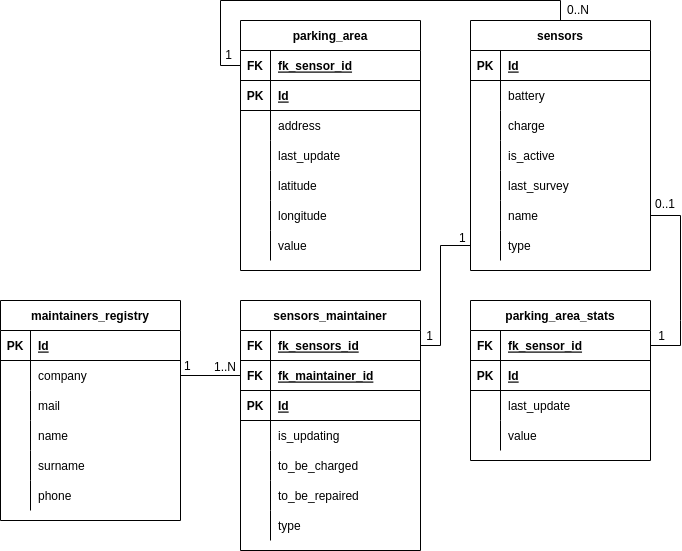
\includegraphics[height=8cm]{modello-logico-vecchio}
\end{figure}

\section{Problemi rilevati}
\textbf{Nomi tabelle incoerenti}
\\\\
I nomi di alcune tabelle erano incoerenti con la funzionalità che andavano a svolgere:
\\\\
sensors\_maintainer è la tabella che contiene i dati di manutenzione dei sensori, un 
nome più appropriato potrebbe essere sensors\_maintenance.
\\\\
parking\_area è la tabella che rappresenta la piazzola di parcheggio, un nome più appropriato
potrebbe essere parking\_spots.
\\\\\\
\textbf{Duplicazione di dati}
\\\\
La tabella parking\_area\_stats non serve a nulla, in quanto duplica soltanto dei dati già presenti
nella tabella parking\_area, creando un'inutile ridondanza di dati.
\\\\\\
\textbf{Cardinalità delle relazioni errata}
\\\\
La relazione sensors -> parking\_area ha cardinalità uno a molti, nel senso che una piazzola può avere
più sensori e un sensore può essere associato solo a una piazzola. 
\\
La cosa è sbagliata, in quanto una piazzola può si avere più sensori associati (un sensore di parcheggio e/o N
sensori ambientali) ma anche un sensore può essere associato a più piazzole; in quanto un sensore ambientale
può ricoprire un area di N piazzole.
\\\\\\
\textbf{Mancanza di tabelle fondamentali}
\\\\
Manca una tabella fondamentale che rappresenti un parcheggio (un insieme di piazzole). 
\\
Tabella molto importante dato che essa ha un indirizzo e una posizione geografica (latitudine e longitudine), 
riconosciute come tali dagli strumenti di navigazione più comuni, come Google Maps. 
\\
Ogni piazzola di uno stesso parcheggio ha una posizione geografica diversa dalle altre piazzole (discostata di qualche 
metro) e potenzialmente diversa da quella del parcheggio. 
\\
Quindi con la struttura vecchia non è possibile ricercare un parcheggio a sistema passando le coordinate del parcheggio di Google
Maps ad esempio e nemmeno identificare un parcheggio.
\\\\\\
\textbf{Database poco modulare}
\\\\
Il valore del sensore di parcheggio viene salvato all'interno della tabella parking\_area (libero/occupato). Questa cosa non crea problemi ora che 
si è deciso, dall'analisi fatta, di salvare solo l'ultima misurazione di un sensore di parcheggio.
\\\\
Se però in futuro si decidesse di salvare uno storico di misurazioni dei sensori di parcheggio (cosa molto probabile che
avvenga e cosa che viene già fatta con i sensori ambientali), con la struttura attuale non è possibile farlo e i costi
per modificare la struttura del database in futuro, con il progetto in produzione da tempo, sarebbero molto più
alti rispetto a farlo adesso.
\\\\
Inoltre l'aggiunta di una tabella per lo storico non ha un impatto negativo sulla struttura del database.
\clearpage
\section{Ristrutturazione}

Il modello logico ristrutturato è il seguente:
\begin{figure}[H]
  \centering
  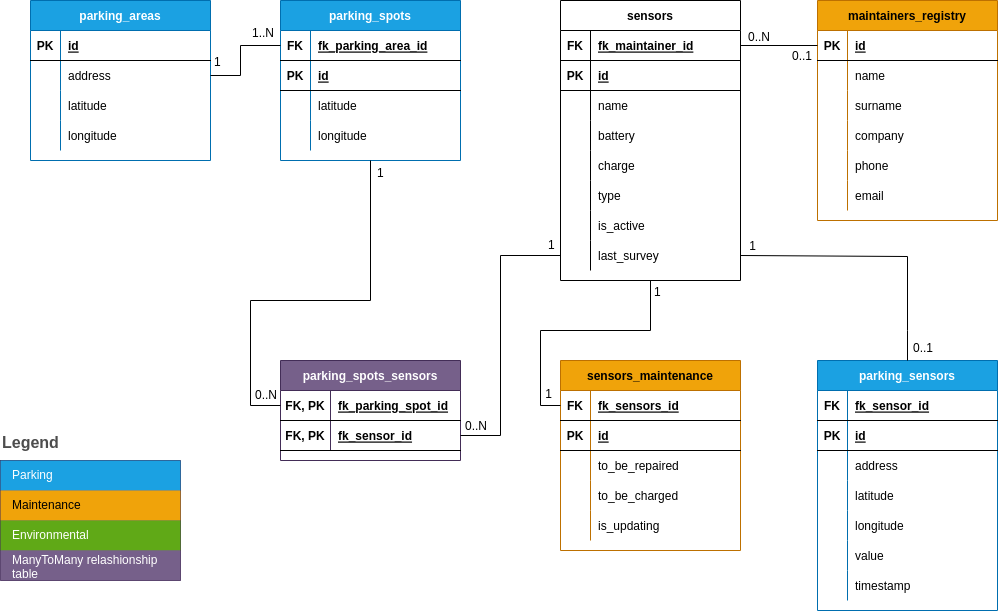
\includegraphics[height=8cm]{modello-logico-ristrutturato}
\end{figure}
\leavevmode\newline
\textbf{Operazioni effettuate:}
\\\\
\textbf{Nomi tabelle incoerenti}
\\\\
Sono stati modificati i nomi di alcune tabelle per renderle più coerenti alla loro funzionalità:
\\\\
parking\_area è stata modificata in parking\_spots.
\\
sensors\_maintainer è stata modificata in sensors\_maintenance.
\\\\
\textbf{Duplicazione di dati}
\\\\
E' stata eliminata la tabella parking\_area\_stats.
\\\\
\textbf{Cardinalità delle relazioni errata}
\\\\
La relazione sensors -> parking\_area è diventata una relazione molti a molti.
\\
E' stato reso facoltativo il fatto che il sensore debba essere associato a una piazzola.
\\
E' stato reso facoltativo il fatto che il manutentore debba essere associato a un sensore.
\\
E' stato reso facoltativo il fatto che il sensore debba essere associato a un manutentore.
\\\\
\textbf{Mancanza di tabelle fondamentali}
\\\\
E' stata aggiunta la tabella parking\_areas che rappresenta i parcheggi, dotati di indirizzo, latitudine e 
longitudine.
\\\\
\textbf{Database poco modulare}
\\\\
E' stata creata la tabella parking\_sensors per salvare la misurazione del sensore di parcheggio ed è
stato tolto il campo value dalla nuova tabella parking\_spots; in quanto avendo già la tabella parking\_sensors,
il campo value rappresentava una ridondanza inutile.
\\\\
Per ogni sensore di parcheggio ora viene salvata solo una misurazione nella tabella parking\_sensors, ovvero
l'ultima, che sovrascrive la precedente ma a differenza del modello logico precedente, se in qualsiasi momento
si decidesse di salvare lo storico delle misurazioni dei sensori di parcheggio, si può fare semplicemente togliendo
il vincolo unique dalla foreign key fk\_sensor\_id della tabella parking\_sensors, senza modificare la struttura delle tabelle.